\documentclass[letterpaper,12pt,fleqn]{article}
\usepackage{matharticle}
\pagestyle{empty}
\documentclass[letterpaper,12pt,fleqn]{article}
\usepackage{matharticle}
\usepackage{graphtheory}
\pagestyle{empty}
\begin{document}

\section*{Graphs}

\begin{definition}[Graph]
  A \emph{graph} is a mathematical object represented by a tuple \(G=G(V,E,\ldots)\) consisting of a set of
  \emph{vertices} (also called \emph{nodes}) \(V=V(G)\), a set of \emph{edges} \(E=E(G)\), and zero of more
  relations.

  Each edge in \(E(G)\) is associated with exactly two (not necessarily distinct) vertices in \(V(G)\) called the
  \emph{endpoints} of the edge.  The nature of the edge/endpoint association is determined by the class of the
  graph (\emph{undirected} vs \emph{directed} and \emph{multi} vs \emph{simple}), which is indicated by the type of
  the elements in \(E(G)\).

  Each relation has \(V(G)\) or \(E(G)\) as its domain and is used to establish additional graph structure or to
  associate vertices or edges with problem-specific attributes (e.g. color, weight).
\end{definition}

\begin{example}
  Graphs are often portrayed visually using filled or labeled circles for the vertices and lines for the edges such
  that each edge line is drawn between its two endpoint vertex circles.
  
  \begin{minipage}[t]{3.25in}
    \vspace{0in}
    \begin{tikzpicture}[node distance=2]
      \begin{scope}[every node/.style=labeled node]
        \node (E) at (0,0) {\(e\)};
        \node (A) [above left=of E] {\(a\)};
        \node (B) [above right=of E] {\(b\)};
        \node (C) [below right=of E] {\(c\)};
        \node (D) [below left=of E] {\(d\)};
      \end{scope}
      \draw (A) edge node [auto] {\(e_1\)} (B);
      \draw (B) edge node [auto] {\(e_2\)} (C);
      \draw (C) edge node [auto] {\(e_3\)} (D);
      \draw (D) edge [bend left] node [auto] {\(e_4\)} (A);
      \draw (D) edge [bend right] node [auto,swap] {\(e_5\)} (A);
      \draw (C) edge [out=345,in=285,min distance=2cm] node [auto] {\(e_6\)} (C);
    \end{tikzpicture}
  \end{minipage}
  \begin{minipage}[t]{2.5in}
    \vspace{0.25in}
    \(V=V(G)=\set{a,b,c,d,e}\)

    \(E=E(G)=\set{e_1,e_2,e_3,e_4,e_5,e_6}\)

    \bigskip

    \begin{tabular}{c|c}
      edge & endpoints \\
      \hline
      \(e_1\) & \(a,b\) \\
      \(e_2\) & \(b,c\) \\
      \(e_3\) & \(c,d\) \\
      \(e_4\) & \(d,a\) \\
      \(e_5\) & \(d,a\) \\
      \(e_6\) & \(c,c\)
    \end{tabular}
  \end{minipage}

  Note that it is not required that all vertices act as endpoints to edges; in the above example, vertex \(e\) is
  such a vertex.
\end{example}

\begin{definition}[Order]
  Let \(G\) be a graph.  The \emph{order} of \(G\), typically denoted by \(n=n(G)\), is the number of vertices in
  \(G\):
  \[n=n(G)=\abs*{V(G)}\]
\end{definition}

\begin{definition}[Size]
  Let \(G\) be a graph.  The \emph{size} of \(G\), typically denoted by \(m=m(G)\), is the number of edges in \(G\):
  \[m=m(G)=\abs*{E(G)}\]
\end{definition}

In the above example, \(n=5\) and \(m=6\).

\begin{definition}[Degenerate Cases]
  \begin{itemize}[left=0in]
  \item[]
  \item The \emph{null} graph is the graph with no vertices \((n=m=0)\).
  \item The \emph{trivial} graph is the graph with exactly one vertex and no edges \((n=1,m=0)\).  Otherwise, the
    graph is \emph{non-trivial}.
  \item An \emph{empty} graph is a graph with no edges \((m=0)\).
  \end{itemize}
  Hence, both the null graph and the trivial graph are empty.
\end{definition}

\begin{definition}[Labeled Graph]
  To say that a graph \(G\) is \emph{labeled} means that its vertices are considered to be distinct and are
  assigned identifying names (labels) by adding a bijective labeling function to the graph tuple:
  \[\ell:V(G)\to L\]
  where \(L\) is a set of labels (names).  Otherwise, the vertices are considered to be identical (only the
  structure of the graph matters) and the graph is \emph{unlabeled}.
\end{definition}

Since the labeling function \(\ell\) is bijective, a vertex \(v\in V(G)\) with label ``a'' can be identified by
\(v\) or \(\ell^{-1}(a)\).  In practice, the presence of a labeling function is assumed for a labeled graph and so
a vertex is freely identified by its label.  This is important to note when a proof includes a phrase such as,
``let \(v\in V(G)\ldots\)'' since \(v\) may be a reference to any vertex in \(V(G)\) or may call out a specific
vertex by its label.  The intention is usually clear from the context.

\end{document}

\end{document}

\DeclarePairedDelimiter{\ceil}{\lceil}{\rceil}
\DeclarePairedDelimiter{\floor}{\lfloor}{\rfloor}
\newcommand{\comp}[1]{\overline{#1}}
\begin{document}
\section*{Decomposition}

\begin{definition}[Decomposition]
  Let $G$ be a simple graph. A \emph{decomposition} of $G$ is a collection of
  simple graphs $G_1,G_2,\ldots G_k$ such that:
  \begin{enumerate}
  \item $E(G)=\bigcup_{k=1}^nE(G_k)$
  \item $\forall\,i,j,E(G_i)\cap E(G_j)=\emptyset$
  \end{enumerate}
\end{definition}

\begin{examples}
  \listbreak
  \begin{enumerate}
  \item $K_4$

    \begin{minipage}{1in}
      \centering
      \gkfour{2}
    \end{minipage}
    \begin{minipage}{0.5in}
      \centering
      $=$
    \end{minipage}
    \begin{minipage}{1in}
      \centering
      \begin{tikzpicture}[scale=2]
        \vertex{a}{(0,0)};
        \vertex{b}{(1,0)};
        \vertex{c}{(1,1)};
        \vertex{d}{(0,1)};
        \draw (a) to (c) to (d) to (a);
        \draw (b) to (c);
      \end{tikzpicture}
    \end{minipage}
    \begin{minipage}{0.5in}
      \centering
      $\bigcup$
    \end{minipage}
    \begin{minipage}{1in}
      \centering
      \begin{tikzpicture}[scale=2]
        \vertex{a}{(0,0)};
        \vertex{b}{(1,0)};
        \vertex{d}{(0,1)};
        \draw (a) to (b);
        \draw (b) to (d);
      \end{tikzpicture}
    \end{minipage}

    \bigskip

  \item $P=5P_4$

    \begin{minipage}{1.5in}
      \centering
      \gpeter{1}
    \end{minipage}
    \begin{minipage}{0.5in}
      \centering
      $=$
    \end{minipage}
    \begin{minipage}{1.5in}
      \centering
      \begin{tikzpicture}
        \vertex{d}{({2*cos(72)+1},{4*sin(72)})};
        \vertex{e}{(0,{2*sin(72)})};
        \vertex{g}{({2*cos(72)+2-cos(54)},0.75)};
        \vertex{i}{({2*cos(72)+1},{4*sin(72)-1})};
        \draw (g) to (i) to (d) to (e);
      \end{tikzpicture}
    \end{minipage}
    \begin{minipage}{0.5in}
      \centering
      $\bigcup$
    \end{minipage}
    \begin{minipage}{1.5in}
      \centering
      \begin{tikzpicture}
        \vertex{c}{({4*cos(72)+2},{2*sin(72)})};
        \vertex{d}{({2*cos(72)+1},{4*sin(72)})};
        \vertex{f}{({2*cos(72)+cos(54)},0.75)};
        \vertex{h}{({4*cos(72)+2-0.75},{2*sin(72)})};
        \draw (f) to (h) to (c) to (d);
      \end{tikzpicture}
    \end{minipage}
    \begin{minipage}{0.5in}
      \centering
      $\bigcup$
    \end{minipage}

    \vspace{0.5in}
    
    \begin{minipage}{1.5in}
      \centering
      \begin{tikzpicture}
        \vertex{b}{({2*cos(72)+2},0)};
        \vertex{c}{({4*cos(72)+2},{2*sin(72)})};
        \vertex{g}{({2*cos(72)+2-cos(54)},0.75)};
        \vertex{j}{(0.75,{2*sin(72)})};
        \draw (c) to (b) to (g) to (j);
      \end{tikzpicture}
    \end{minipage}
    \begin{minipage}{0.5in}
      \centering
      $\bigcup$
    \end{minipage}
    \begin{minipage}{1.5in}
      \centering
      \begin{tikzpicture}
        \vertex{a}{({2*cos(72)},0)};
        \vertex{b}{({2*cos(72)+2},0)};
        \vertex{f}{({2*cos(72)+cos(54)},0.75)};
        \vertex{i}{({2*cos(72)+1},{4*sin(72)-1})};
        \draw (b) to (a) to (f) to (i);
      \end{tikzpicture}
    \end{minipage}
    \begin{minipage}{0.5in}
      \centering
      $\bigcup$
    \end{minipage}
    \begin{minipage}{1.5in}
      \centering
      \begin{tikzpicture}
        \vertex{a}{({2*cos(72)},0)};
        \vertex{e}{(0,{2*sin(72)})};
        \vertex{h}{({4*cos(72)+2-0.75},{2*sin(72)})};
        \vertex{j}{(0.75,{2*sin(72)})};
        \draw (a) to (e) to (j) to (h);
      \end{tikzpicture}
    \end{minipage}
  \end{enumerate}
\end{examples}

\begin{definition}[Path Number]
  Let $G$ be a simple graph. The \emph{path number} for $G$, denoted $p(G)$, is
  the minimum number of paths in any decomposition of $G$.
\end{definition}

\newpage

\begin{conjecture}[Gallai]
  Let $G$ be a simple graph of order $n$. $G$ can be decomposed into at most
  $\ceil*{\frac{n}{2}}$ paths. In other words:
  \[p(G)\le\ceil*{\frac{n}{2}}\]
\end{conjecture}

\begin{example}
  Since $n(P)=10$, so $p(P)\le\ceil*{\frac{10}{2}}=5$, meaning the Petersen
  graph can be decomposed into at most $5$ paths --- indeed: $P=5P_4$ as shown
  above and $p(P)=5$, but we need a way to find a lower bound.
\end{example}

\begin{theorem}
  Let $G$ be a simple graph. If $G$ can be decomposed into $k$ paths then the
  number of odd vertices in $G\le2k$.
\end{theorem}

\begin{theproof}
  Assume $G$ can be decomposed into $k$ paths:
  \[G=\bigcup_{i=1}^kP_{n_i}\]
  Isolated vertices are treated as $P_1$ and are considered even. Each of the
  other paths consist of $2$ odd vertices and $n_i-2$ even vertices:

  \begin{tikzpicture}
    \vertex{a}{(0,0)} node at (a) [below] {$o$};
    \vertex{b}{(1,0)} node at (b) [below] {$e$};
    \node (c) at (2,0) {};
    \node (d) at (3,0) {};
    \vertex{e}{(4,0)} node at (e) [below] {$e$};
    \vertex{f}{(5,0)} node at (f) [below] {$o$};
    \draw (a) to (b) to (c);
    \draw (d) to (e) to (f);
    \node at (2.5,0) {$\cdots$};
  \end{tikzpicture}

  Let $G_i$ be the spanning subgraph of $G$ such that $E(G_i)=E(P_{n_i})$, in
  other words, $G_i$ contains the vertices and edges from $P_{n_i}$ and all of
  the remaining vertices in $G$ as isolated vertices. For example, if $G=K_4$,
  one such $G_i$ might be:

  \begin{tikzpicture}
    \vertex{a}{(0,0)};
    \vertex{b}{(2,0)};
    \vertex{c}{(2,2)};
    \vertex{d}{(0,2)};
    \draw (a) to (b) to (d);
  \end{tikzpicture}

  consisting of a $P_3$ and one isolated vertex.

  Let $e(G_i)$ be the number of even (including isolated) vertices in $G_i$ and
  $o(G_i)$ be the number of odd vertices in $G_i$:
  \[\bigcap_{i=1}^ke(G_i)\subseteq e(G)\]
  The LHS contains all isolated vertices in $G$ and all vertices that are
  either isolated or in the interior of the path in each $G_i$. Note that a
  vertex that is in the interior of multiple paths (never an end vertex of a
  path) remains even:

  \begin{tikzpicture}
    \node (a) at (0,0) {};
    \node (b) at (0,2) {};
    \node (c) at (2,2) {};
    \node (d) at (2,0) {};
    \vertex{e}{(1,1)};
    \draw (a) to (e) to (c);
    \draw (b) to (e) to (d);
  \end{tikzpicture}

  However, the LHS is a subset of the RHS, because two end (odd) vertices in
  different paths can be joined in $G$ to form an even vertex:
  
  \begin{tikzpicture}
    \node (a) at (0,0) {};
    \vertex{b}{(1,0)};
    \node (c) at (2,0) {};
    \draw (a) to (b) to (c);
  \end{tikzpicture}

  But no even vertex on the LHS can be converted to an odd vertex, because it
  would have to be an end vertex in at least one path and thus would not be in
  the LHS:

  \begin{tikzpicture}
    \node (a) at (0,2) {};
    \vertex{b}{(0,1)};
    \node (c) at (0,0) {};
    \node (d) at (1,1) {};
    \draw (a) to (b) to (c);
    \draw (b) to (d);
  \end{tikzpicture}
\end{theproof}

Now, take the complement of both sides:
\[\comp{\bigcap_{i=1}^ke(G_i)}\supseteq\comp{e(G)}=o(G)\]
To see why this is true, consider the following Venn diagram for $V(G)$:

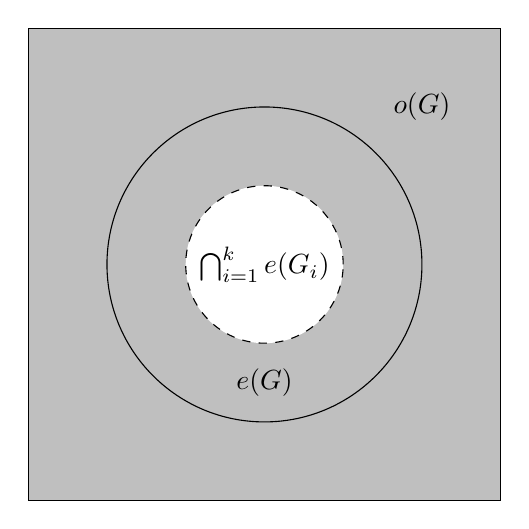
\begin{tikzpicture}
  \draw [fill=lightgray] (0,0) rectangle (6,6);
  \draw (3,3) circle [radius=2];
  \draw [dashed,fill=white] (3,3) circle [radius=1];
  \node at (5,5) {$o(G)$};
  \node at (3,1.5) {$e(G)$};
  \node at (3,3) {$\bigcap_{i=1}^ke(G_i)$};
\end{tikzpicture}

Now, applying DeMorgan:
\[o(G)\subseteq\comp{\bigcap_{i=1}^ke(G_i)}=\bigcup_{i=1}^k\comp{e(G_i)}=
\bigcup_{i=1}^ko(G_i)\]
And then the triangle inequality:
\[\abs{o(G)}\le\abs{\sum_{i=1}^ko(G_i)}\le\sum_{i=1}^k\abs{o(G_i)}=
\sum_{i=1}^k2=2k\]

$\therefore\abs{o(G)}\le2k$

\begin{examples}
  \listbreak
  \begin{enumerate}
  \item P

    By Gallai: $p(P)\le5$. By the lemma: $10\le2p(P)$ and so $p(P)\ge5$.
    Therefore $p(P)=5$. A decomposition $P=5P_4$ is shown above.

  \item $C_n$

    $P(C_n)=P_n\cup P_2$ and so $p(C_n)=2$

  \item $ST_n$

    $ST_{2k+1}=\bigcup_{i=1}^kP_3$ and so $p(ST_{2k+1})=k$

    $ST_{2k}=\bigcup_{i=1}^{k-1}P_3\cup P_2$ and so $p(ST_{2k})=k$

    Therefore: $p(ST_n)=\floor*{\frac{n}{2}}$
  \end{enumerate}
\end{examples}

\end{document}
